\section{M = 0 D}
\begin{center}
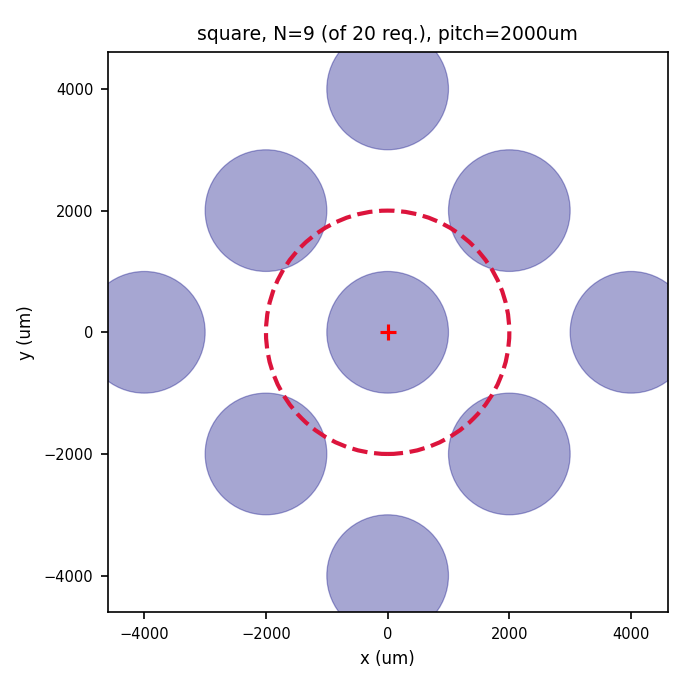
\includegraphics[width=0.55\textwidth]{winner_viz_figs/fig_M0.png}
\end{center}
\texttt{ring\_offset\_concentric}, ring\_spacing=1000\,$\mu$m, N=11,
a\_hole=2000\,$\mu$m. Margin 1.000/1.000 --- passes with real (not structural)
margin. Blind rate 15.6\%.

\section{M = 1 D}
\begin{center}
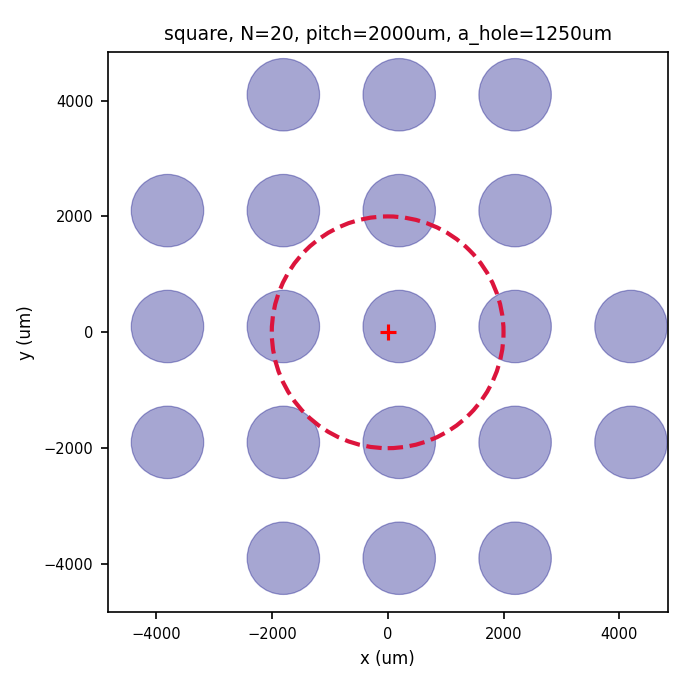
\includegraphics[width=0.55\textwidth]{winner_viz_figs/fig_M1.png}
\end{center}
\texttt{square}, pitch=2000\,$\mu$m, N=20, a\_hole=1250\,$\mu$m. Margin
0.128/0.128 --- the one finite-margin design in this set. Blind rate 8.2\%,
the lowest of any winner.

\section{M = 2--3 D}
\begin{center}
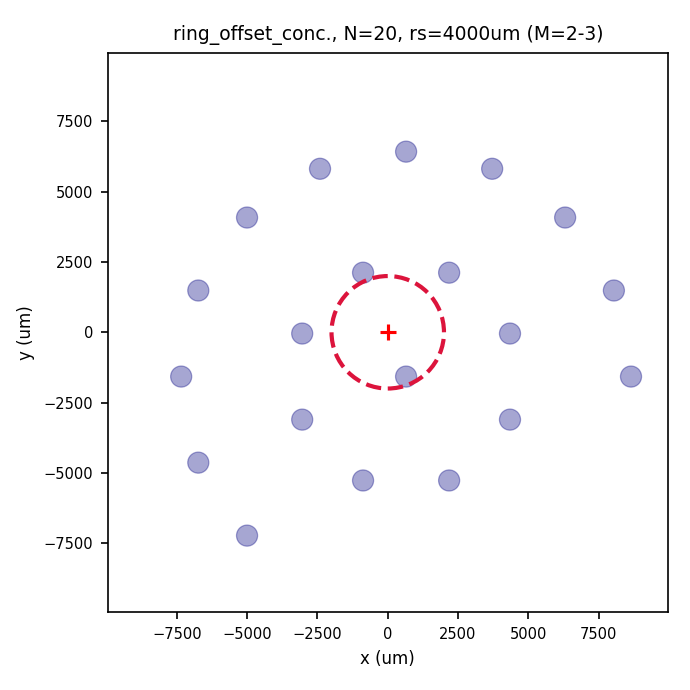
\includegraphics[width=0.55\textwidth]{winner_viz_figs/fig_M2_3.png}
\end{center}
\texttt{ring\_offset\_concentric}, ring\_spacing=4000\,$\mu$m, N=20,
a\_hole=750\,$\mu$m. Margin $+\infty$ (structurally ghost-free). Blind rate
$\sim$10.7\%.

\newpage
